\chapter{Inference from the 21cm signal}

\begin{bf}
  \author{Bradley Greig}\\
  
Abstract\\
\end{bf}

The 21cm signal is physics rich and encodes a wealth of astrophysical and cosmological information (refer back to previous chapters here). However, how do we extract this information? This chapter focusses on how we intend to extract the interesting physics from the observed 21cm signal.

Essentially, the problem can be broken down into three parts:
\begin{itemize}
\item[1.] Compressing the observed data into a manageable dataset (i.e. statistic or images) to tease out the interesting physics. Which is the optimal statistic, and what in particular is it optimal for?
\item[2.] An efficient means to model/simulate the 21cm signal
\item[3.] A robust probabilistic framework to compare simulations to observations to extract the physics.
\end{itemize}
\noindent
In this chapter we will focus on each separately, before concluding with the current state of the art in inference of the 21cm signal.

\section{What do we actually measure?}

Ultimately, we observe the brightness temperature fluctuations in the 21cm signal, relative to the background CMB temperature. In effect, we observe $\delta T_{b,\rm 21cm}(\nu,\mathbf{x})$, dependant on the observed frequency (line of sight distance) and the 2D angular position on the sky. Interferometric experiments (e.g.) enable us to access the full 3D information of the 21cm signal. Global experiments on the other hand average out the brightness temperature over the entire sky, compressing the information into a single average brightness as a function of frequency.

Once we have a measurement of this 3D 21cm signal, we are free to compress the data in an innumerable number of ways. We can extract single 2D tomographic images of the differential brightness temperature as a function of redshift (frequency) enabling us to be able to directly observe the topology of the neutral and ionised gas during reionisation. Alternatively we can average out the 3D information either spatially or in frequency to maximise the signal to noise in a certain regime to maximise certain astrophysical processes and features expected during reionisation.

\section{Optimal methods for extracting the astrophysics and cosmology from the 21cm signal}

To infer the interesting astrophysics and cosmology from the observational data, we need a way to characterise the spatially and time varying 21cm signal. The signal is weak, therefore we likely will need to compress the data in some way to tease out the interesting physics from the noise.

Here, list a variety of known ways in which can be used to extract information about the 21cm signal. This will include both imaging and statistical techniques. For each, provide a brief discussion about the method (i.e. what it is) and then what leverage it provides in regard to the astrophysics etc. and what specific features are useful \textbf{(this may marginally overlap with Jordan's section on Predictions and Challenges)}. At various points in this section, can refer back to previous chapters when specific physics is being referred to. For example, if a specific statistic is sensitive to a certain population of sources or an epoch of history, refer back to the appropriate section in the previous chapters.

This should be a considerable more in-depth discussion that what is covered in Jordan's and Jonathan Pritchard's chapters. Need to gauge the overlap between these chapters.

\textbf{Need to work in Adrian Liu's paper highlighting the importance of knowing $\tau$ for precision recovery of cosmology}

\subsection{Minkowski functionals}

Compresses the information down into a single number, which can describe the connectedness and overall topology of the 21cm signal. Cite Zaroubi, also a recent arXiv paper (Chen maybe).

\subsection{Global signal}

Describes the entire globally averaged history of the 21cm signal. Turning points/features within the signal can be used to disentangle information about sources etc. Can also throw in some discussion regarding EDGES/DM, i.e. fundamental cosmology + astrophysics. \textbf{How much overlap is there going to be between this and Jordan/Jonathan Pritchard's chapters.?}

There are a variety of papers investigating the global signal. Could be a few different ways to use the signal to extract information. \textbf{This may overlap with Jordan's chapter on predictions and challenges.}

\subsection{Power spectrum}

The main goto statistic to describe the signal. Sensitive to a vast array of astrophysics. \textbf{This may overlap with Jordan's chapter on predictions and challenges.}

However, doesn't fully describe the signal. Power spectrum is a Gaussian statistic, the signal is inherently non-Gaussian. Therefore information loss.

This should focus only on the 3D spherically averaged 21cm PS. Can mention that the 2D cylindrically averaged PS can in principle also be used, and why it would be useful.

\subsection{Skewness/Kurtosis/PDFs etc.}

A means to measure the non-Gaussianity of the signal, however, compresses the information as it is a scale independent quantity. Useful for describing topology and evolution of the signal. Has certain characteristic features of interest. See Catherine's paper and others.

\subsection{Bispectrum}

A scale dependant measure of the non-Gaussianity of the 21cm signal. Superior to both the power spectrum and skewness etc.. More complicated to visualise/understand. Has been used to describe the EoR quite extensively. Discuss the variety of configurations and their utility/usefulness. See Suman's, and other publications.

\subsection{Wavelets}

An alternative to simply Fourier transforming the data, a family of wavelets can be used to transform the 21cm data to a more useful basis. For example, the Morlet transform allows the transform to be localised both in frequency and in space, improving over the Fourier transform which can only be localised in one or the other. 

In theory, it should contain similar, if not more information that the power spectrum, as it can disentangle line-of-sight effects better. See Cath's paper.

\subsection{Individual bubbles}

Images will provide a direct tangible link to the process of reionisation. Revealing exactly where ionising bubbles are, and thus where to look for the sources responsible for the bubble creation. 

However, bubble identification will become rather problematic, as it is the differential brightness that is observed, not the raw brightness temperature. Need smart/sophisticated approaches to search and characterise the signal.

Look at individual regions of interest, i.e. around a bright QSO or large number of galaxies. 

Matched filters etc., are useful for finding/detecting isolated bubbles

\subsection{Stacked images}

May be difficult to detect individual objects, instead, one could stack 21cm spectra centred on known galaxies. See Paul Geil's paper.

Border's on potential discussions of synergies. Requires known locations of ionising sources with precise redshifts and positions of the sky. JWST/WFIRST. Is there 

\subsection{Bubble size distributions/statistics}

Constructing a statistical distribution of the ionised bubbles through redshift can reveal information about the size and number of galaxies responsible for reionisation (also the production rate of the ionising photons).

Techniques to recover statistical distributions are for example Sambit's super pixels stuff. Need to look at Koki's granulometry stuff to see where that sits in this context.

\subsection{Other statistics}

Are there other statistics that I have overlooked/forgotten. Need to do a search of the literature to ensure I have covered everything.

\section{Efficient methods to model/simulate the 21cm signal}

Ideally we want to use the largest, most physically accurate simulations to match the observed 21cm signal. However, this is not practical. Instead, we must come up with methods to compensate accuracy for efficiency.\\
\\
Originally I envisaged this section to go as follows
\begin{itemize}
\item Discuss briefly that numerical simulations are great but too computationally expensive
\item Highlight semi-numerical/analytic simulations as fitting the bill by being faster etc.
\item Then discuss alternatives (i.e. emulators).
\end{itemize}
This will need to be re-worked given Jordan's plan to discuss this. I haven't yet thought of a logical plan to motivate this. I guess one way would be to concatenate it into just a simulation section and briefly summarise what was discussed in Jordan's chapter (which is a couple of chapters ago, so might be appropriate to do so). It's less obvious to move into discussing emulators in the absence of motivating the need for them by highlighting the complications of simulations in general.

\subsection{Numerical simulations}

Ideally, use large, numerical simulations to make a realisation which matches observation. Want to include as much physics as possible into these simulations. Doing so, comes at a serious cost. Simulating the 21cm signal is complicated! Brief summary on the required dynamic range. Briefly highlight the expensive nature of these simulations, Hydrodynamics, radiative transfer etc. Quickly becomes computationally prohibitive to run more than a couple of realisations. \textbf{Jordan's section (Modelling Tools) will likely cover most if not all of this}.

\subsection{Semi-numerical/analytic models of the 21cm signal}

Enter semi-numerical approaches, which broadly encapsulate the global average quantities of reionisation and the cosmic dawn and reproduce morphologically similar realisations of the 3D structure. The advantage here is that the computational costs are drastically reduced (orders of magnitude less). \textbf{Jordan's section (Modelling Tools) will likely cover most if not all of this}.

\subsection{Intelligent sampling of the parameter space}

Running simulations to span all of the allowed parameter space may be too computationally intensive. However, perhaps we can make intelligent assumptions/guesses about how many simulations to run, and on a specific area of physics to focus on. Some of the concepts here may overlap slightly with the Emulator section below. This sampling was discussed in one of Benoit's recent papers.

\subsection{Emulators}

An alternative to directly running a simulation to estimate some astrophysical statistic/model, one can instead construct a function which estimates what the statistical signal should be, given some astrophysical or cosmological parameter set. This is what is referred to as an emulator. Using simulations, a generator function is constructed which can approximate the statistics of the signal. Results in multiple orders of magnitude improvement in computational speed as no new simulations are required. However, it can only approximate statistics, it does not generate 3D simulations. 

Developing an emulator benefits from efficient parameter space approaches, as it minimises the size of the database required to construct the emulator. There are a variety of approaches to consider when attempting to minimise the sampling of the astrophysical parameter space. For example Latine-Hypercube, Gaussian processes... Can briefly discuss each method, and a few recent papers that explore methods to do this

There are numerous machine learning approaches to construct an emulator.

Discuss Nick Kern's of 21cmFAST and Cohen's global signal one of Anastasia's code.

\subsection{Characterising our ignorance}

We are fully aware that semi-numerical approaches are inaccurate at 10s of per cent level. Additionally, they oversimplify/completely ignore the underlying astrophysical properties. However, if the global quantities (observables such as luminosity functions etc.) can still be reproduced within agreement, we can develop an understanding of how one might map from a semi-numerical simulation, to a more realistic simulation. Basically, tell the large, computationally expensive simulation where exactly to look in the region of parameter space.

Using summary statistics and globally average observables, we can develop a means to calibrate one simulation to mimic the outputs of another. In other words, develop a bias or functional form to smooth out uncertainties from one simulation to mimic the results of a more detailed simulation.

Describe ongoing attempts to quantify this. i.e. use luminosity functions to calibrate simulations, apply redshift corrections to deal with photon non-conservation etc.

These correction factors etc., will be crucial for inferring astrophysics and cosmology from the 21cm signal


\section{Inference methods for 21cm}

Having discussed methods to model/simulate the 21cm signal, now need to shift focus to methods to infer information about the astrophysics/cosmology from the 21cm signal.

\subsection{Fisher Matrices}

Simplest method, which takes derivatives with respect to model parameters of a functional form (i.e. a 21cm statistical signal) to infer parameter constraints. Effectively, exploits how sensitive the 21cm signal is to specific parameters. Limiting assumption include Gaussianity etc.

Successfully used for cosmology

\subsection{Bayesian MCMC}

Significantly more robust method to parameter inference. Outline Bayes' theorem. Highlight that this basically boils down to exploring by random walks, using a likelihood function and priors to accept/penalise regions of parameter space. Very useful for recovering constraints. Again, successfully used in Cosmology etc.

Describe its use in the context of 21cm. Introduce 21CMMC, and a couple of other codes that use MCMC (Sultan's simfast21, Jordan's global signal, Geraint's MCMC, Simon's Mhysa). Highlight that 21CMMC is the only direct MCMC. Emphasise that techniques such as emulators can be coupled with MCMC to improve overall computational efficiency at the cost of some further inaccuracies.

\subsection{Nested sampling and model inference}

We have a wide variety of simulations, each with their own strength's and weaknesses. In principle, various models/simulations/physical prescriptions can be discriminated against using model selection or inference. Related to MCMC, nested sampling can focus on model selection rather than simply astrophysical recovery. Can refer to Tom Binnie's recent paper.

\subsection{Neural Networks}

Instead of using MCMC to recover parameters from statistics, we can use the full 2/3D images of the 21cm signal with neural networks. One can construct a database of simulations and extract the 21cm signal to construct a neural network. This network can then learn an large number of properties, i.e. how changes in the topology are affected by astrophysical parameters etc. Using this technique one can directly convert from an observed 2D image to the underlying astrophysics. Like emulators, the application of the network is extremely quick. Downsides are parameter errors etc. and in some sense physical intuition. It tells you an answer, but not why.

Simulated images of the 21cm signal have already been used to infer astrophysical and cosmological constraints. For example with convolutional networks (e.g Nicolas or Paul La Plante). Discuss other machine learning approaches.



\iffalse

Lorem ipsum dolor sit amet, consectetur adipiscing elit. Duis eu egestas erat. Maecenas tincidunt lacinia tincidunt. Mauris id lectus nec neque feugiat condimentum vitae at diam. In vel orci nunc, non commodo mauris. Vivamus ipsum enim, vulputate quis pharetra non, molestie quis felis. Vivamus porttitor placerat turpis at accumsan. Nunc tortor velit, faucibus a rhoncus nec, blandit non elit. Nam consectetur lectus eu nisi blandit dapibus rhoncus dui tempus. Mauris fermentum dolor vel ipsum vulputate sit amet ultricies tortor lacinia. Donec ut nibh erat. Morbi nec mi ante. Integer nec vestibulum diam. Donec tincidunt pellentesque quam, ut interdum mauris venenatis condimentum. Nam condimentum, augue in aliquet gravida, neque dui elementum eros, id semper eros purus sed felis. Curabitur in justo sit amet sapien ultrices hendrerit at quis nibh. Quisque iaculis pulvinar tincidunt. 
\begin{eqnarray}
C(12) &= &\left[\overrightarrow{\pi}\cdot\overrightarrow{\phi}(x+r)\right] \nonumber \\ 
&\approx& 1-\mathrm{const}\frac{r^2}{L^2}\int_r^L\frac{x\rmd x}{x^2} + \cdots \nonumber  \\
&\approx& 1-\mathrm{const}\frac{r^2}{L^2}\ln\frac{x\rmd x}{x^2} + \cdots .\label{brokenlongeqn}
\end{eqnarray}

Aenean tellus risus, porta sit amet porta vitae, tincidunt ut felis. Class aptent taciti sociosqu ad litora torquent per conubia nostra, per inceptos himenaeos. Vestibulum ante ipsum primis in faucibus orci luctus et ultrices posuere cubilia Curae; Phasellus pulvinar placerat velit auctor egestas. Vivamus euismod fringilla tincidunt. Sed ut magna felis, id sollicitudin nunc. Quisque a dui eu erat consectetur egestas a quis justo. Aenean euismod congue diam, vel posuere urna fermentum sit amet. Lorem ipsum dolor sit amet, consectetur adipiscing elit. Mauris faucibus lacus eget est mollis auctor. Donec at nibh ligula, et posuere massa. Phasellus quis leo diam \cite{diamantaras1996pcn}.
Donec aliquam blandit risus, eu venenatis ante euismod eu. Curabitur cursus justo id arcu condimentum feugiat. Integer sapien urna, vulputate et adipiscing nec, convallis et justo. Suspendisse in ipsum at felis ornare interdum \cite{tulone2006pts},

\begin{figure}[]
\begin{center}
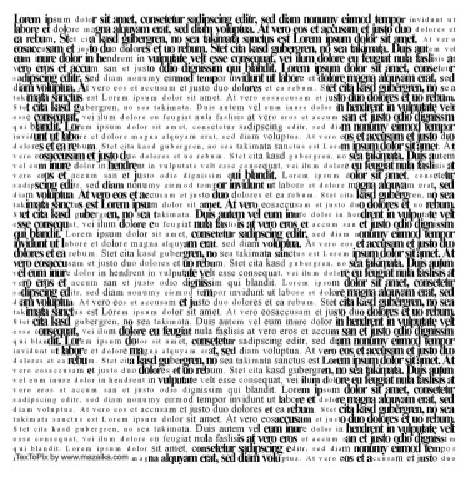
\includegraphics[width=0.5\textwidth]{Greig/01x01-eps-converted-to}
\end{center}
\caption{This is figure 1 in chapter 1.}
\end{figure}

\paragraph{Cras adipiscing} sagittis nunc vel luctus. Suspendisse volutpat augue quis erat semper consequat dignissim tellus euismod. Morbi hendrerit, tellus id aliquam iaculis, nibh leo tincidunt eros, vitae varius ligula felis in mi.

\begin{table}
\caption{Greek Letters.}
\begin{center}
\begin{tabular}{llllllll}
\hline
$\alpha $  & $ \beta $  & $ \gamma $  & $ \delta $  & $ \epsilon $  & $ \varepsilon $  & $ \zeta $  & $ \eta $ \\
 $ \theta $  &  $ \vartheta $  &  $ \gamma $  &  $ \kappa $  &  $ \lambda $  &  $ \mu $  &  $ \nu $  &  $ \xi $ \\
 $ o $  &  $ \pi $  &  $ \varpi $  &  $ \rho $  &  $ \varrho $  &  $ \sigma $  &  $ \varsigma $  &  $$ \\
 $ \tau $  &  $ \upsilon $  &  $ \phi$ &  $ \varphi $  &  $ \chi $  &  $ \psi $  &  $ \omega$  &  $ $ \\
 &  &  &  &  &  &  & \\
$ \Gamma $  & $ \Delta $  & $ \Theta $  &  $ \Lambda $  &  $ \Xi $  &  $ \Pi $  &  $ \Sigma $  & $ \Upsilon $ \\
 $ \Phi$ &  $ \Psi $  &  $ \Omega $  &  &  &  &  &\\
\hline
\end{tabular}
\end{center}\end{table}

\begin{figure}[]
\begin{center}
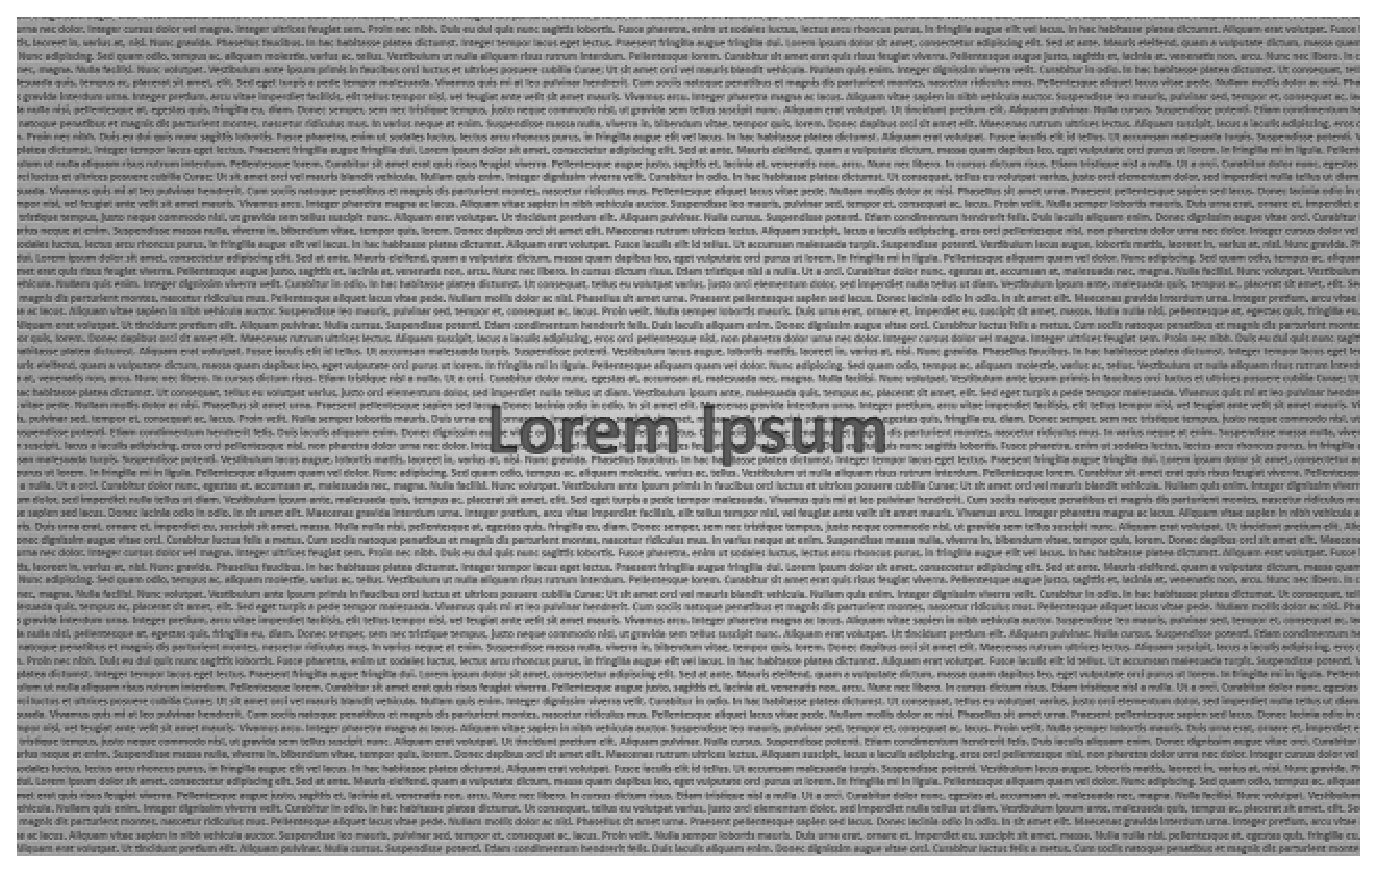
\includegraphics[width=0.6\textwidth]{Greig/01x02}
\end{center}
\caption{This is figure 2 in chapter 1.}
\end{figure}

\fi

\bibliographystyle{plain}
\bibliography{Greig/References}


